% !TEX TS-program = pdflatex
% !TEX encoding = UTF-8 Unicode

% This is a simple template for a LaTeX document using the "article" class.
% See "book", "report", "letter" for other types of document.

\documentclass[11pt]{article} % use larger type; default would be 10pt

\usepackage[utf8]{inputenc} % set input encoding (not needed with XeLaTeX)

%%% Examples of Article customizations
% These packages are optional, depending whether you want the features they provide.
% See the LaTeX Companion or other references for full information.

%%% PAGE DIMENSIONS
\usepackage{geometry} % to change the page dimensions
\geometry{a4paper} % or letterpaper (US) or a5paper or....
\geometry{margin=1in} % for example, change the margins to 2 inches all round
% \geometry{landscape} % set up the page for landscape
%   read geometry.pdf for detailed page layout information

\usepackage{graphicx} % support the \includegraphics command and options

% \usepackage[parfill]{parskip} % Activate to begin paragraphs with an empty line rather than an indent
\usepackage{amssymb}
\usepackage{amsmath}
%%% PACKAGES
\usepackage{booktabs} % for much better looking tables
\usepackage{array} % for better arrays (eg matrices) in maths
\usepackage{paralist} % very flexible & customisable lists (eg. enumerate/itemize, etc.)
\usepackage{verbatim} % adds environment for commenting out blocks of text & for better verbatim
\usepackage{subfig} % make it possible to include more than one captioned figure/table in a single float
% These packages are all incorporated in the memoir class to one degree or another...

%%% HEADERS & FOOTERS
\usepackage{fancyhdr} % This should be set AFTER setting up the page geometry
\pagestyle{fancy} % options: empty , plain , fancy
\renewcommand{\headrulewidth}{0pt} % customise the layout...
\lhead{}\chead{}\rhead{}
\lfoot{}\cfoot{\thepage}\rfoot{}

%%% SECTION TITLE APPEARANCE
\usepackage{sectsty}
\allsectionsfont{\sffamily\mdseries\upshape} % (See the fntguide.pdf for font help)
% (This matches ConTeXt defaults)

%%% ToC (table of contents) APPEARANCE
\usepackage[nottoc,notlof,notlot]{tocbibind} % Put the bibliography in the ToC
\usepackage[titles,subfigure]{tocloft} % Alter the style of the Table of Contents
\usepackage{bbm}
\usepackage{endnotes}

\renewcommand{\cftsecfont}{\rmfamily\mdseries\upshape}
\renewcommand{\cftsecpagefont}{\rmfamily\mdseries\upshape} % No bold!
\DeclareMathOperator*{\argmax}{arg\,max}
\DeclareMathOperator*{\argmin}{arg\,min}

\usepackage{graphicx}
\graphicspath{ {./pings/} }

\newcount\colveccount
\newcommand*\colvec[1]{
        \global\colveccount#1
        \begin{pmatrix}
        \colvecnext
}
\def\colvecnext#1{
        #1
        \global\advance\colveccount-1
        \ifnum\colveccount>0
                \\
                \expandafter\colvecnext
        \else
                \end{pmatrix}
        \fi
}

\newcommand{\norm}[1]{\left\lVert#1\right\rVert}

\title{Computational Problem Set 3}
\author{Michael B. Nattinger, Sarah J. Bass, Xinxin Hu}

\begin{document}
\maketitle

\section{Dynamic Programming Problem}

First we solve for the agents optimization problem given prices $w,r$ and benefits $b$. First I will derive the labor supply equation; after I present figures of decision rules, and finally I solve for general equilibrium and construct table 1 and discuss the solutions.

A working age household chooses $a',l$ to solve their value function:
\begin{align*}
V_{j}(a,z) &= \max_{a'\geq 0, l}\{ u^w(w(1-\theta)e(z,\eta_j)l + (1+r)a - a',l) + \beta E[V_{j+1}(a',z')] \}
\end{align*}

Taking FOCs wrt labor:
\begin{align*}
(1-\sigma) U_w^{\frac{-\sigma}{1-\sigma}}[\gamma c^{\gamma - 1}(1-l)^{1-\gamma}we(1-\theta) - (1-\gamma)c^{\gamma}(1-l)^{-\gamma}] &= 0 \\
\Rightarrow c &= \frac{\gamma (1-l)we(z,\eta_j)(1-\theta)}{1-\gamma} 
\end{align*}

We can write out the budget constraint and use our FOC to plug in for c:
\begin{align*}
(1-\theta)wle(z,\eta_j) &= c + a' - (1+r)a \\
(1-\theta)wle(z,\eta_j) &= \frac{\gamma (1-l)we(z,\eta_j)(1-\theta)}{1-\gamma}  + a' - (1+r)a \\
(1-\theta)wle(z,\eta_j)(1-\gamma) &= \gamma (1-l)we(z,\eta_j)(1-\theta)  + (1-\gamma)(a' - (1+r)a) \\
(1-\theta)wle(z,\eta_j) &= \gamma we(z,\eta_j)(1-\theta)  + (1-\gamma)(a' - (1+r)a)\\
l &= \frac{ \gamma we(z,\eta_j)(1-\theta)  + (1-\gamma)(a' - (1+r)a)}{(1-\theta)we(z,\eta_j)}.
\end{align*}
Here we have the desired expression. Plots are below.

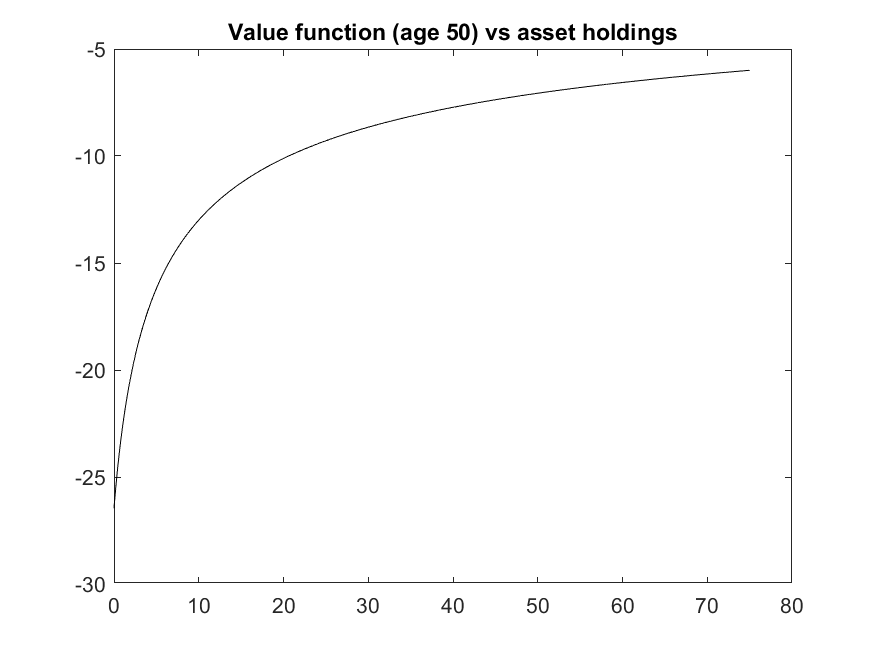
\includegraphics{value}

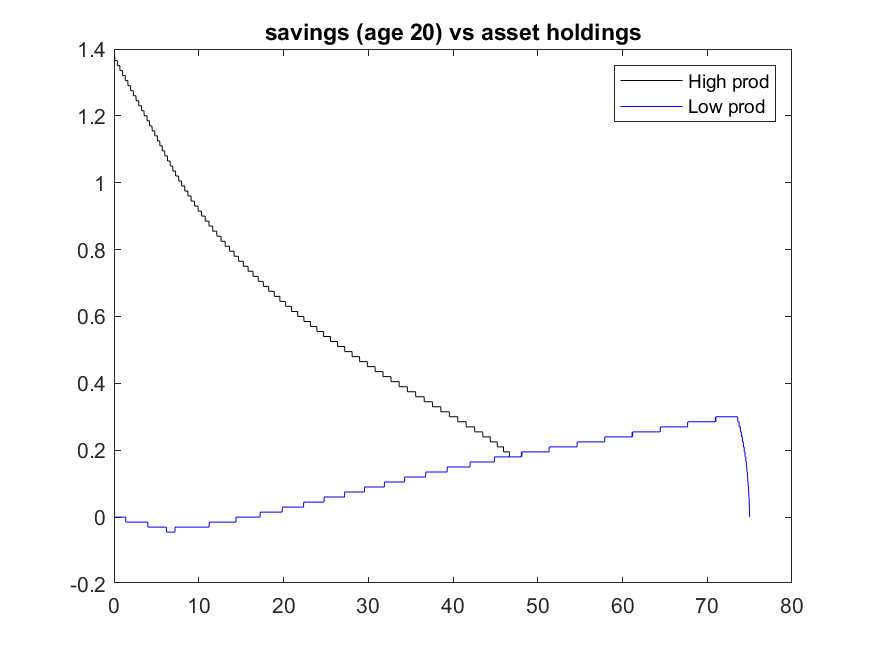
\includegraphics{savings}

Above we have our value function for retired agents of age 50, note it is concave and increasing. We also have our savings function for agents at age 20. Note that savings is decreasing in assets for high productivity workers (but always above zero). For low productivity workers with a very small number of assets, savings is decreasing in assets, while for higher levels of assets the low productivity workers have savings increasing in asset holdings. Note that near the right end of the asset grid these functions are a bit funky - keep in mind that no agents populate these regions.

Now we compute GE models to endogenize our prices. To summarize our results, we refer to table 1 below:

\begin{center}
\begin{tabular}{ll}
& beta \\ 
\hline 
education & 0.14431 \\ 
experience & 0.042633 \\ 
experience\^{}2/100 & -0.095056 \\ 
constant & 0.53089 \\ 
\hline 
\end{tabular}
\end{center}

We now address the three questions posed to us, answering by referring to table 1:
\begin{enumerate}
\item Our economy is dynamically efficient because $n<r$. By setting $\theta = 0$, capital rises as households save more for retirement (as now they receive no retirement benefits). Higher capital increases the marginal product of labor, which results in increased wages and therefore higher levels of labor. People end off worse off (as measured via welfare) because the retirement benefits served to insure those who could no longer work (the elderly); without it, the households will work more to insure their future selves (who deterministically will end up in this retired state at some point in the future). The winners of this reform are the productive young, as they avoid taxes under the reform, and therefore generate more income to be spent on consumption and savings while young. The losers are the unproductive young, who are likely to have lower wealth when old than the productive young (and then would have more to gain from the benefits due to the concavity of their utility function), and the old (who directly receive the benefits transfers).
\item With no risk, the aggregate capital stock falls significantly. This is because less effective labor is supplied by the households, due to the mechanically lower productivities of the households. Capital is then less productive, and also the households have less labor income so the capital supply falls dramatically. There is no need to save in precaution of getting hit with a low productivity shock in the future, as all workers have low productivity so there is no 'non-low' state. In this case, when social security is taken away almost nothing happens to welfare - it is hardly unchanged from the model with social security (Note: clearly we are supposed to say something along the lines of what I wrote but I really caution against taking this too literally. Utility is an ordinal ranking, we really cannot say that the utility without social security is 'hardly unchanged' just because the level of utility without social security is close to the level without it - all we can say is that welfare is lower without social security). What is going on here is that, without idiosyncratic uncertainty, agents are almost indifferent about whether they would like to save for retirement themselves or have the government "save" for them (through retirement benefits). In contrast, with idiosyncratic uncertainty (as in our base case), agents much prefer the government insure them as the agents are very bad off if they have to insure themselves and happen to face a bad stream of productivity shocks (due to concavity of utility). 
\item When labor supply is exogenous, capital shoots up because more output is produced, capital is more productive, and benefits shoot up. Without social security, capital shoots up even more as agents save for retirement. The labor tax which funds social security was distortive under the benchmark model, but here there is no distortion as labor is inelastically supplied. In other words, the negative aspect of social security (the distortionary impact on labor supply) disappears with inelastic utility, and only the positive insurance benefits remain. Without social security, households feel the negative impact from the lack of pension benefits without receiving any of the benefits from the removal of the distortionary labor tax, so in this case the removal of social security is worse relative to the baseline case.
\end{enumerate}
\end{document}
